\documentclass{article} 
\usepackage[left=0.75in,top=0.6in,right=0.75in,bottom=0.6in]{geometry} % Document margins
\usepackage{tabularx}
\usepackage{fancyvrb}
\usepackage{graphicx}
\usepackage{multicol,caption}
\usepackage{fancyhdr}
\usepackage{lipsum}
\usepackage{mathtools}
\usepackage{float}

%Header Stuff
\newenvironment{Figure}
  {\par\medskip\noindent\ignorespaces\minipage{\linewidth}}
  {\endminipage\par\medskip}

\usepackage{fancyhdr}
\pagestyle{fancy}
\fancyhf{}
\renewcommand{\headrulewidth}{0pt}
\fancyhead[R]{\thepage}


\begin{document}

%----------------------------------------------------------------------------------------
%		 TITLE 
%----------------------------------------------------------------------------------------
\begin{center}

\vspace* {15 pt}
\Huge{\bf Creating  a Graphical User Interface(GUI) for processing images }\\
\vspace {20 pt}
\large{Howard Edwards, Michael Micros, Jonathon  Rigney, Megan Rowland \\}

\end{center}

\vspace{20 pt}




\begin{multicols*}{2}

%----------------------------------------------------------------------------------------
%		ABSTRACT
%----------------------------------------------------------------------------------------
{\bf  \textit {Abstract(Howard Edwards)} ---
}\\
     This report covers the development of a graphical user interface, GUI, used for image processing. The graphical user interface allows for the reading and writing of 8-bit grayscale images for processing. Image processing done by the GUI is image overlaying, histogram equalization, and the image adjustment of brightness and contrast. After the completion of image processing, the interface displays the processed images. The GUI was designed to facilitate the constant viewing of inputted images and their outputs while processes are being performed.  All image processing is initiated completely via the interface’s widgets and results displayed simultaneously. 


{\bf  \textit {Index Terms} --- Gray-scale, Image analysis, Image processing
}



%----------------------------------------------------------------------------------------
%		INTRODUCTION
%----------------------------------------------------------------------------------------

\begin{center}
\large{I. Introduction(Jonathon Rigney)}
\end{center}

 The goal of this report is to explain the results of the second milestone of a larger project for an integrated system that performs the processing of real-time video through an user-interface on a computer. The completed system incorporates the use of field-programmable gate arrays, FPGA’s.
     Presented is a detailed documentation outlining the results of developing a graphical user interface that will allow its users to read and write images, perform image overlay, histogram equalization, along with brightness and contrast adjustments on the images. Users can load and display 8-bit original images and overlay images. Original images that are processed by overlaying can be displayed alongside its original form for comparison. Processed images can also be displayed through histogram equalization.
     The program for performing image processing is written in C++. As this is the case, the framework for the graphical user interface must support C++.  The framework used to develop the graphical user interface was the Qt application. Qt is a cross-platform software development framework that enables the creation, building and deployment of embedded devices and application.




%----------------------------------------------------------------------------------------
%		DESIGN
%----------------------------------------------------------------------------------------

\begin{center}
{\large II. Design (Michael Micros)}
\end{center}

{\bf A. Summary of Design--}  

The overall design consists of a Qt program that provides a GUI with which the user will interact. The GUI contains several buttons, each of which performs a specific action. These actions include loading in and saving images, performing histogram equalization and overlaying the uploaded image with another image of the user's choice. Finally, the design also incorporates sliders that allow for the adjustment of image contrast and brightness. The result of each action is displayed in a separate label on the GUI, as can be seen in the Figure below

\begin{Figure}
 \centering
 \includegraphics[width=\linewidth]{GUI.png}
  \captionof{figure}{Layout of the GUI: top left=original image, bottom left= equalized, top center=overlay image, bottom center overlay result, top right=contrast adjusted image, bottom right=brightness adjusted image.}
\end{Figure}

{\bf B. Detail Description}\\

{\bf Loading an Image:}  
In order to load an image to the GUI, the “Choose and Image” button must be clicked. By programming the following action into the button the user is prompted to select an image.


\begin{Figure}
 \centering
 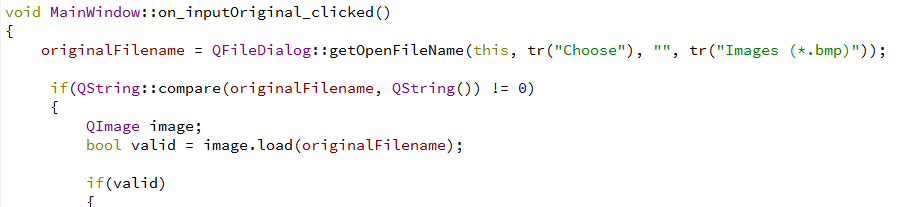
\includegraphics[width=\linewidth]{inputimage.png}
  \captionof{figure}{Code that promts user to select an Image and loads it to a QImage object}
\end{Figure}


The QImage object is then displayed in the Label object which allows it to be visible to the user.


\begin{Figure}
 \centering
 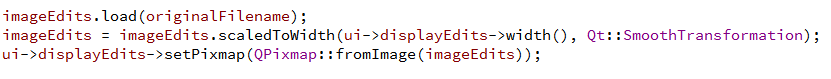
\includegraphics[width=\linewidth]{labelDisplay.png}
  \captionof{figure}{Code that displays image on GUI using Label object}
\end{Figure}



A similar process is used whenever it is necessary to display an image in the GUI.

{\bf Histogram equalization:} 
Upon loading in an image, the histogram equalization of that image is performed automatically according to the method used in the paper by Edwards et al [1] (Milestone 1 Report). Also the maximum and minimum pixel values of the uploaded image are calculated. These values will be used in adjusting the brightness and contrast of the image.

{\bf Overlaying:} 
In order to perform image overlaying, an action is assigned to the “Choose and Overlay Image” button on the GUI. When pressed, the user will be prompted to select an image to be overlaid on the original image that the user has already uploaded. Upon selecting the image, the image overlay process takes place according to  Edwards et al [1].The result of that function is “out1.bmp”, which is automatically loaded and displayed in the proper label.

{\bf Contrast adjustment using Slider widget:} 
The slider widget has a signal named “value changed” which is activated whenever the slider is moved. The slider represents a value from 0 to 99 with 0 being all the way left and 99 being all the way to the right. To calculate the changes in contrast to each pixel in the image as the slider is moved to the left or right the following formula is used:\\
\[\text{newPV }= \]
\[ \frac{ \text{newMin+ (newMax-newMin)}   \times  \text{(origPix - oldMin)}}{\text{(oldMax-oldMin)}} \] \\
where 
imageEdits.pixel(i, j) = original image pixel value,
newPV = contrast changed pixel,
newMin = minimum pixel value in the new range,
newMax = maximum pixel value in the new range,
oldMin = minimum pixel level in the original image,
oldMax = maximum pixel level in the original image.
          
The newMinLevel and the newMaxLevel proportionally increase as the slider is moved to the right and decreases as the slider is moved to the left. This allows the contrast of the image to be enhanced by utilizing a greater range of pixel values and vice versa lessen by utilizing a smaller range of pixel values. If the range of pixel values are greater than 50 to 205, the newMinLevel is set to 50 and the newMaxLevel is set to 205. This allows an increase in range of pixel by one for each increment of the slider. 

{\bf Brightness adjustment using Slider widget:} 
Similarly to the contrast adjustment, the value of the slider is used to calculate the new value of each pixel in the image to be displayed. The overall objective is to add a certain value to each image pixel according to the position of the slider (and consequently the value that it represents). As can be seen in the Figure below, the constant value that is added to all pixels is described by the equation: 
\[ \text{change =  } \frac{  value \times (maxLevelOrigImage -minLevelOrigImage) }{50}\]

\begin{Figure}
 \centering
 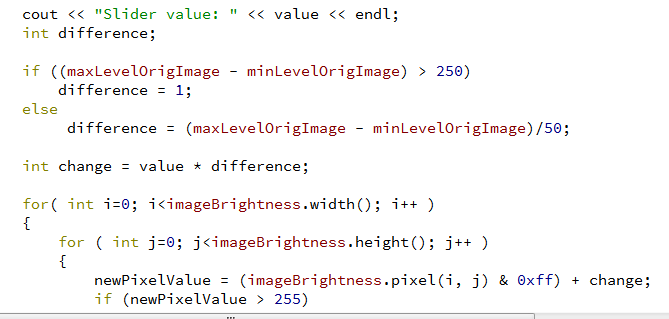
\includegraphics[width=\linewidth]{brightnessadjustment.png}
  \captionof{figure}{Code demonstrating the process of brightness adjustment}
\end{Figure}


{\bf Saving an image:} 
In similar fashion to uploading an image, saving an image is performed by clicking the button that corresponds to the image (Label object) to be saved to file.This is accomplished using the Qimage::save() function that requires the filename, format and quality factor to be specified. All images are saved in appropriately named files, specifically :  "HistogramEqualizedImage.bmp", "OverlaidImage.bmp", "ContrastEditsImage.bmp", "BrightnessEditsImage.bmp".


%----------------------------------------------------------------------------------------
%		EVALUATION
%----------------------------------------------------------------------------------------

\begin{center}
{\large III. Evaluation (Megan Rowland)}\\
\end{center}

\begin{Figure}
 \centering
 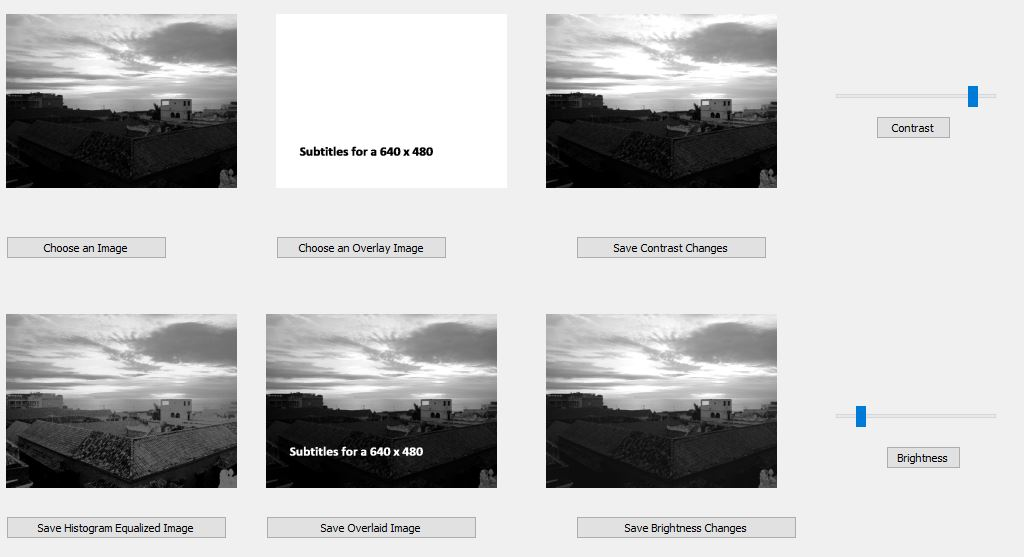
\includegraphics[width=\linewidth]{Image2GUI.jpg}
  \captionof{figure}{Complete GUI layout after loading Image and performing all functions}
\end{Figure}


The program functions and produces the outcomes as expected.

First, the GUI allows the user to load an 8-bit bitmap original image. Once the user clicks on the “Choose an Image” button and selects the image, the original image loads in the view above the button:

\begin{Figure}
 \centering
 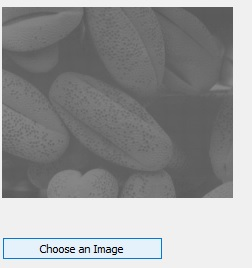
\includegraphics[width=\linewidth]{OriginalImage.jpg}
\end{Figure}

\begin{Figure}
 \centering
 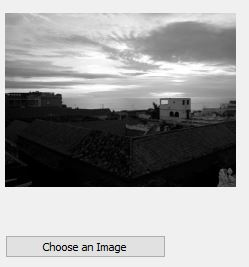
\includegraphics[width=\linewidth]{OriginalImage2.jpg}
\end{Figure}

Second, the GUI allows the user to load an 8-bit bitmap overlay image. Once the user clicks on the “Choose an Overlay Image” button and select the image, the overlay image loads in the view above the button:


\begin{Figure}
 \centering
 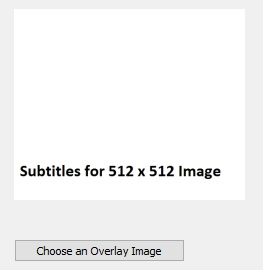
\includegraphics[width=\linewidth]{OverlayImage.jpg}
\end{Figure}

\begin{Figure}
 \centering
 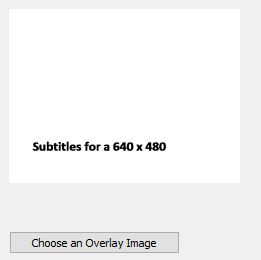
\includegraphics[width=\linewidth]{OverlayImage2.jpg}
\end{Figure}

Third, the GUI generates and displays, below the overlay image load function, an image by overlaying the overlay image over the original image. Below the image is a button to “Save Overlaid Image” to a file. Clicking on this button saves the overlaid image:


\begin{Figure}
 \centering
 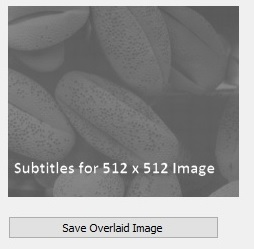
\includegraphics[width=\linewidth]{OverlaidImage.jpg}
\end{Figure}

\begin{Figure}
 \centering
 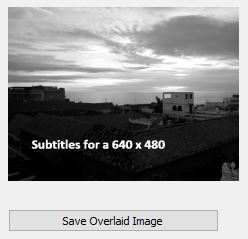
\includegraphics[width=\linewidth]{OverlaidImage2.jpg}
\end{Figure}

Fourth, the GUI generates and displays an image from the histogram equalization of the original image. Below the image is a button to “Save Histogram Equalized Image” to a file. Clicking on this button saves the histogram equalized image:


\begin{Figure}
 \centering
 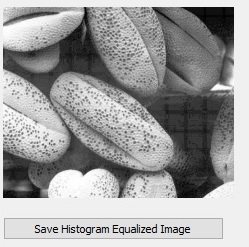
\includegraphics[width=\linewidth]{HistogramEqualizedImage.jpg}
\end{Figure}

\begin{Figure}
 \centering
 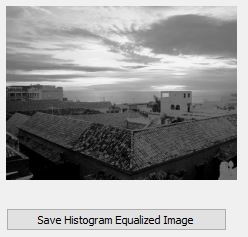
\includegraphics[width=\linewidth]{HistogramEqualizedImage2.jpg}
\end{Figure}

Fifth, the GUI offers a slider to adjust the brightness of the original image. Move the slider to manually adjust the contrast of the original image. Below the image is a button to “Save Brightness Changes” to a file. Click on this button saves the changes in a brightness file. As can be seen below, when the slider is moved to the left the brightness decreases and when the slider is moved to the right the brightness increases.


\begin{Figure}
 \centering
 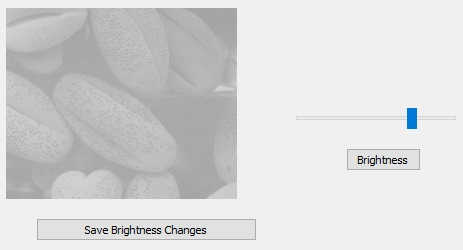
\includegraphics[width=\linewidth]{BrightnessImage.jpg}
\end{Figure}

\begin{Figure}
 \centering
 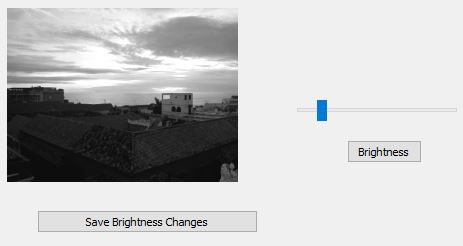
\includegraphics[width=\linewidth]{BrightnessImage2.jpg}
\end{Figure}

Sixth, the GUI offers a slider to adjust the contrast of the original image. Move the slider to manually adjust the contrast of the original image. Below the image is a button to “Save Contrast Changes” to a file. Clicking on this button saves the changes in contrast to a file. As can be seen below, the contrast of the image decreases when the slider is moved to the left and the contrast increases as the slider is moved to the right.

\begin{Figure}
 \centering
 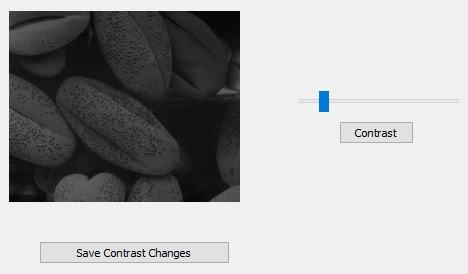
\includegraphics[width=\linewidth]{ContrastImage.jpg}
\end{Figure}

\begin{Figure}
 \centering
 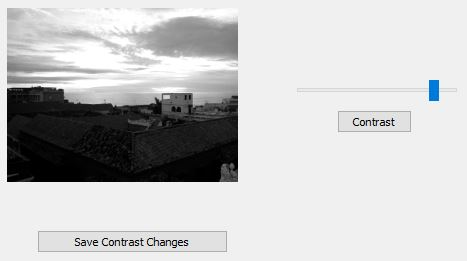
\includegraphics[width=\linewidth]{ContrastImage2.jpg}
\end{Figure}


\vspace{15 pt}

%----------------------------------------------------------------------------------------
%		DISCUSSION
%----------------------------------------------------------------------------------------


\begin{center}
{\large IV. Discussion (Megan Rowland)}
\end{center}

Based on the results in the Evaluation section, the GUI functions as expected. There is not much room for improvement for the GUI. The layout is self explanatory, all of the different functions respond very quickly, and the images are large enough to view efficiently without taking up too much landscape. 
The contrast and brightness sliders seem to work best with an image that occupies a limited range of values (for example 160 to 230) rather than the entire 255 length spectrum.
One way in which to improve the GUI is to make the layout a bit easier on the eye, but that will be left up to the Human Factors team to optimize. Also more effective algorithms to perform the contrast adjustment could be implemented, but the speed of the application may be negatively impacted. 

%----------------------------------------------------------------------------------------
%		APPENDIX
%----------------------------------------------------------------------------------------


\begin{center}
{\large V. Appendix}
\end{center}

\end{multicols*}













%----------------------------------------------------------------------------------------
\end{document}
